% !TeX spellcheck = en_GB
%==============================================================================
% Voorbeeld gebruik documentklasse hogent-article
%==============================================================================
%
% Compileren in TeXstudio:
%
% - Zorg dat Biber de bibliografie compileert (en niet Biblatex)
%   Options > Configure > Build > Default Bibliography Tool: "txs:///biber"
% - F5 om te compileren en het resultaat te bekijken.
% - Als de bibliografie niet zichtbaar is, probeer dan F5 - F8 - F5
%   Met F8 compileer je de bibliografie apart.
%
% Als je JabRef gebruikt voor het bijhouden van de bibliografie, zorg dan
% dat je in ``biblatex''-modus opslaat: File > Switch to BibLaTeX mode.

\documentclass{hogent-article}

%images
\usepackage{graphicx}
\graphicspath{ {./img/} }

%------------------------------------------------------------------------------
% Metadata over het artikel
%------------------------------------------------------------------------------

%---------- Titel & auteur ----------------------------------------------------

% TODO: geef werktitel van je eigen voorstel op
\PaperTitle{Hebben de factoren feedback en locatie invloed op de resultaten van de retrieval practice studiemethode?}
% TODO: geef op welk soort artikel dit is
% Dit is typisch de opdracht en het vak waarvoor dit artikel geschreven is, bv.
\PaperType{Verslag onderzoeksproject Onderzoekstechnieken 2018-2019}

% TODO: vul je eigen naam in als auteur, geef ook je emailadres mee!
\Authors{Olivier Troch\textsuperscript{1}, Daan Van Vooren\textsuperscript{2}, Robbie Verdurme\textsuperscript{3}, Sebastien Wojtyla\textsuperscript{4}} % Authors

% TODO: vul de naam van je co-promotor in.
% Als het hier gaat om een voorstel voor de bachelorproef, dan ben je hier
% verplicht de naam van je co-promotor in te vullen. Zoniet, dan kan je het
% leeg laten.
\CoPromotor{}

% Contactinfo: Geef hier de contactgegevens van elke auteur van het artikel
\affiliation{
	\textsuperscript{1} \href{mailto:olivier.troch.w2257@student.hogent.be}{Olivier.troch.w2257@student.hogent.be}
}
\affiliation{
	\textsuperscript{2} \href{mailto:daan.vanvooren.y1502@student.hogent.be}{daan.vanvooren.y1502@student.hogent.be}
}
\affiliation{
	\textsuperscript{3}
	\href{mailto:robbie.verdurme.y9234@student.hogent.be}{robbie.verdurme.y9234@student.hogent.be}
}
\affiliation{
	\textsuperscript{4}
	\href{mailto;sebastien.wojtyla.y3274@student.hogent.be}{sebastien.wojtyla.y3274@student.hogent.be}
}

%---------- Abstract/Samenvatting ----------------------------------------------------------
\Abstract{In deze paper wordt onderzocht wat de effecten zijn op de resultaten van de retrieval practice studiemethode. In veel studies werd reeds aangetoond dat retrieval practice een goede studiemethode is maar welke factoren invloed hebben is minder besproken. Deze paper gaat dieper in op deze vraag door te onderzoeken of het krijgen van feedback en de locatie gedurende de retrieval practice methode invloed hebben op de resultaten. De verwachte resultaten zijn dat zowel feedback als de locatie een positief effect zal hebben en dus betere testresultaten zal opleveren. Deze paper kan bijdragen aan verder onderzoek van de retrieval practice methode.
}

%---------- Onderzoeksdomein en sleutelwoorden --------------------------------
% TODO: Vul de sleutelwoorden aan.
\Keywords{Onderzoeksproces, Studiemethodes, Retrieval Practice}
\newcommand{\keywordname}{Sleutelwoorden} % Defines the keywords heading name

%---------- Titel, inhoud -----------------------------------------------------
\begin{document}
	
	\flushbottom % Makes all text pages the same height
	\maketitle % Print the title and abstract box
	\tableofcontents % Print the contents section
	\thispagestyle{empty} % Removes page numbering from the first page
	
	%------------------------------------------------------------------------------
	% Hoofdtekst
	%------------------------------------------------------------------------------
	
	\section{Inleiding}
	Retrieval practice is een studiemethode die ervoor zorgt dat leerstof langer onthouden kan worden op lange termijn. Hoewel reeds aangetoond is dat dit een effectieve methode is voor het studeren verwachten wij een ander resultaat wanneer we enkele variabelen aanpassen. Eén van de variabelen die we zullen testen in deze paper is de locatie waar gestudeerd wordt en de invloed hiervan op het studeren. 
	Een andere variabele die mogelijks ook invloed heeft op de efficiëntie van deze studiemethode is het geven van feedback tussen de verschillende test iteraties.
	
	\section{Literatuurstudie}
%Retrieval practice
	Er zijn veel verschillende methoden om te studeren. Eén van deze methoden is de retrieval practice methode. Hierbij wordt gefocust op het continu heropvragen van leerstof door middel van testen. Dit zou een positief effect hebben op het onthouden van de leerstof op lange termijn.
    Verschillende artikels \autocite{butler2010repeated, pyc2012test, karpicke2007repeated, karpicke2008critical} hebben deze methode al uitbundig bestudeerd. In deze studies test men vier verschillende methodes. De eerste methode is de studie-test-studie-test methode (STST), dit is de standaard retrieval practice methode waarbij het studeren wordt gevolgd door het afleggen van een test en dit twee maal. Eén week later volgt de finale test waarin de resultaten worden bekeken. De drie andere methoden zijn SSSS, SSST en STTT die op analoge manier worden uitgevoerd.
	Tussen deze methoden werd een groot verschil waargenomen op het langetermijngeheugen. De standaard STST methode resulteerde in het beste resultaat waarbij de testpersoon de leerstof na één week tijd nog grotendeels kon reconstrueren. Het slechtste resultaat werd waargenomen bij de SSSS methode die beduidend minder goed scoorde dan de andere methodes waarin wel getest werd. Hieruit kunnen we afleiden dat het testen een belangrijke rol speelt tijdens het studeren. Wat echter nog onduidelijk is, is welke factoren het resultaat van de retrieval practice methode kunnen beïnvloeden. Deze paper probeert een antwoord te bieden op deze vraag. Met behulp van verschillende artikels die zich binnen de context van deze vraag bevinden zal een hypothese worden opgesteld.
    
    
%Feedback geven     
    Een eerste artikel \autocite{brame2015test} beschrijft enkele variabelen die het resultaat van een test kunnen beïnvloeden. Eén van deze variabelen is het geven van feedback na een test. Uit de resultaten bleek dat personen die feedback kregen na de eerste test over het algemeen minder kans hadden om dezelfde fout te maken in een tweede test.
    In een ander artikel \autocite{roediger2011critical} wordt verder ingespeeld op deze variabele. Hierbij wordt onderzocht of de tijdstippen waarop een tester feedback krijgt invloed heeft. Er werden drie scenario's onderzocht: het krijgen van feedback direct na de test, uitgesteld feedback krijgen of helemaal geen feedback krijgen. Het resultaat was dat testers die direct feedback kregen beter scoorden in een tweede afgelegde test. Deze variabele zal verder onderzocht worden in deze paper.
    
    Een andere variabele die in het artikel \autocite{brame2015test} getest wordt is de importantie voor het behalen van een goed resultaat. De conclusie was dat een test die grote invloed heeft op het verdere levensverloop van de tester veel belangrijker is en dus ook de drijfveer van de tester positief beïnvloedt.
    
    Een andere studie \autocite{karpicke2009metacognitive} onderzocht hoe studenten presteren wanneer ze niet verplicht zijn om de retrieval practice methode toe te passen. Eén groep gebruikte verplicht de retrieval practice methode en een andere groep kon zelf kiezen hoe ze studeerden: retrieval practice, blijven studeren of verder gaan wanneer ze denken dat ze de leerstof beheersen. Uit de resultaten bleek dat studenten die zelf mochten kiezen minder goede resultaten behaalden. Ze kozen minder vlug voor de retrieval practice methode omdat ze dachten dat ze de leerstof beheersten terwijl dit niet het geval was. 
    
    
%Plaats
    Een laatste variabele dat invloed kan hebben op de testresultaten is de locatie waar gestudeerd wordt en waar de test wordt afgelegd. Uit verschillende artikels \autocite{smith1978environmental, smith1984contextual} kan afgeleid worden dat het brein zich aan verschillende omgevingen moet aanpassen waardoor deze meer gestimuleerd wordt. Daarbij zal het brein ook de studiematerie kunnen linken aan de omgeving waarin gestudeerd word en zo makkelijker de nieuwe materie kan onthouden. Deze variabele zal ook onderzocht worden in deze paper.
      

%Verschillende onderwerpen studeren
    Naast al deze variabelen is het ook niet onbelangrijk aan te halen dat een andere studiemethode ook invloed kan hebben op het onthouden van leerstof op lange termijn. Zo bestaat er een studiemethode genaamd interleaved practice. Deze wordt gebruikt wanneer meerdere onderwerpen gestudeerd moeten worden. Hierbij zullen deze verschillende onderwerpen door elkaar gestudeerd worden in plaats van elk onderwerp apart te studeren (= blocking practice). Uit een studie \autocite{taylor2010effects} bleek dat interleaved practice een beduidend beter testresultaat opleverde. Interleaved practice kan ook gecombineerd worden met retrieval practice, dit zou tot een nog beter resultaat kunnen leiden van de retrieval practice studiemethode, maar deze combinatie zal in deze paper niet verder onderzocht worden aangezien deze buiten de scope valt van het onderzoek.
    
	
	\section{Variabelen}    
    De variabelen die getest worden in deze paper zijn feedback en locatie tijdens de retrieval practice methode.
    De eerste variabele die invloed kan hebben op het resultaat is het geven van feedback na een test. Dit kan een grote invloed hebben op het studeren zoals reeds bewezen is \autocite{roediger2011critical, brame2015test}.
    Door het geven van feedback weet de testpersoon welke fouten hij/zij gemaakt heeft. Vervolgens kan de testpersoon rekening houden met deze feedback tijdens een volgende studie iteratie. Hierdoor zullen eerder gemaakte fouten minder snel voorkomen in volgende test iteraties.
    
    De tweede variabele die onderzocht wordt in deze paper is de locatie waar gestudeerd wordt en waar de test wordt afgenomen. Dit is omdat het brein zich aan verschillende omgevingen moet aanpassen waardoor deze meer gestimuleerd wordt. Daarbij zal het brein ook de studiematerie kunnen linken aan de omgeving waarin gestudeerd wordt en zo makkelijker de nieuwe materie kan onthouden.
    
    \section{Verwachtingen}
    Tijdens het onderzoek krijgt iedere informatica student een tekst die hij/zij zal moeten bestuderen. Vervolgens wordt de groep opgesplitst in drie subgroepen. Elke subgroep zal de standaard retrieval practice methode (STST) toepassen waarvan twee subgroepen met een aangepaste variabele.
    De eerste subgroep zal de standaard retrieval practice methode toepassen zonder aangepaste variabele. 
    De tweede subgroep zal tussen verschillende studie iteraties verplaatst worden naar een andere locatie waar ook de standaard retrieval practice zal toegepast worden.
    De laatste subgroep zal tijdens het studeren feedback krijgen op de resultaten van hun voorgaande test.
    
    Hierdoor kan nagegaan worden of de variabelen een invloed hebben op het studeren van een tekst aan de hand van de retrieval practice methode. Merk op dat we elke tweedejaars informatica student er toe verplichten om deel te nemen aan deze test waardoor het resultaat niet op de hele groep studenten toepasbaar is zonder enig foutpercentage \autocite{karpicke2009metacognitive}.
    
    We veronderstellen dat de eerste subgroep analoge resultaten zal behalen aan de resultaten uit de artikels over de retrieval practice methode \autocite{butler2010repeated, pyc2012test, karpicke2007repeated, karpicke2008critical}. Dit is omdat deze methode reeds vaak getest werd in verschillende experimenten.
    Daarnaast verwachten we ook dat zowel het geven van feedback als aanpassen van de locatie een positief effect zal hebben op het resultaat en waarbij het geven van feedback het grootste effect zal hebben.
    
    %grafiek feedback apart en locatie apart
    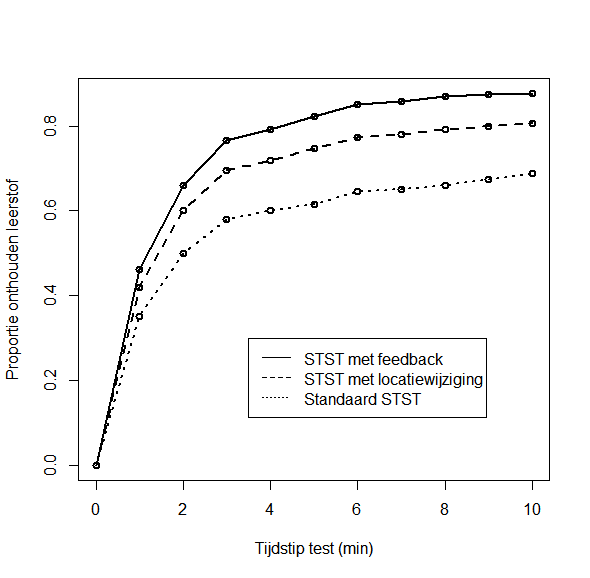
\includegraphics[scale=0.5]{mockGrafiek1}
    
    %onze uitleg
    Door de feedback kan de leerstof beter opgenomen worden. Dit is doordat de testpersoon zich bewust is van zijn/haar gemaakte fouten. Terwijl de locatiewijziging enkel het brein stimuleert maar niet de gemaakte fouten aankaart. Hierdoor hebben deze fouten een grotere kans om opnieuw gemaakt te worden in volgende testen.
    
	%------------------------------------------------------------------------------
	% Referentielijst
	%------------------------------------------------------------------------------
	% TODO: de gerefereerde werken moeten in BibTeX-bestand ``bibliografie.bib''
	% voorkomen. Gebruik JabRef om je bibliografie bij te houden en vergeet niet
	% om compatibiliteit met Biber/BibLaTeX aan te zetten (File > Switch to
	% BibLaTeX mode)
	
	\phantomsection
	\printbibliography[heading=bibintoc]
	
\end{document}
